\section{Material und Methoden} % (fold)
    \label{sec:material_und_methoden}
    % Erhalt numerischer Vektoren
    \subsection{Grundalgorithmus} % (fold)
        \label{sub:grundalgorithmus}
        \newcommand{\PhantomSubSub}[1]{
            \phantomsection
            % \addtocounter{subsubsection}{1}
            % \addcontentsline{toc}{subsubsection}{\protect\numberline{\thesubsubsection} #1}}
            \addcontentsline{toc}{subsubsection}{#1}}
        \begin{algorithm}
            \caption{Übersetzen einer Aminosäuresequenz in einen numerischen Vektor}\label{alg:vorbereitung}
            \PhantomSubSub{Übersetzen einer Aminosäuresequenz in einen numerischen Vektor}
            \newcommand{\I}{\text{\textquotesingle}}
            \begin{algorithmic}
                \Require $sequence \in \{ \text{A-Z}, \I\Psi\I, \I\Omega\I, \I\Phi\I, \I\zeta\I, \I\Pi\I, \I\text{+}\I, \I\text{-}\I\}^{*} $
                \Require $0 \leq kf \leq 10$
                \Ensure $|aa\_vector| = |sequence|$
                \Ensure $v \geq 0\ \forall\ v \in aa\_vector$ 

                \State $aa\_vector \gets \texttt{array}()$
                \ForEach{$aa$}{$sequence$}
                    \State $kf\_value \gets \texttt{get\_kf\_value}(aa, kf)$
                    \State $min\_kf\_value \gets \texttt{get\_min\_kf\_value}()$
                    \State $aa\_vector.\texttt{append}(kf\_value + \texttt{abs}(min\_kf\_value))$
                \EndFor
            \end{algorithmic}
        \end{algorithm}
        Voraussetzung für den Algorithmus ist ein numerischer Vektor, so wie es das Spektrum einer Tonspur bei SHAZAM darstellt. Um dies im Kontext von Proteinen zu erreichen, wird in \protfin\ auf sogenannte Kidera-Faktoren zurückgegriffen. Diese Faktoren stammen aus einem Forschungsprojekt von Akinori Kidera, welches 1985 publiziert wurde. Inhalt des Projekts war die statistische Faktorenanalyse von 188 physikalischen Eigenschaften der 20 natürlichen Aminosäuren zur Ermittlung von 10 dieser Eigenschaften, durch die die anderen aufgrund hoher Korrelation erklärt werden können \vgl{kidera}. In \autoref{tab:kidera} sind diese dargestellt.

        \begin{table}[h]
            \centering
            \caption{Kidera-Faktoren}
            \newcommand{\T}[1]{\centerIt{\textbf{#1}}}
            \label{tab:kidera}
            \csvreader[tabular=lllllllll,
              table head=\toprule\T{Beschreibung} & \T{A} & \T{C} & \T{D} & \T{E} & \T{F} & \T{G} & \textbf{\dots}\\\midrule,
              head to column names,
              late after line=\\,
              late after last line=\\\bottomrule
              ]%
              {../../prot-fin/materials/Amino_Acid_Kidera_Factors.csv}{Kidera_Factor=\KF, Kidera_Factor_Description=\KFD}%
            {\KFD & \A  & \C & \D & \E & \F & \G & \dots}
        \end{table}

        \newpage
        Folglich kann eine Aminosäuresequenz pro Faktor in einen numerischen Vektor übersetzt werden, wobei ein höherer absoluter Wert für mehr Relevanz des Faktors steht. Hätte man also die Beispielsequenz \texttt{EVKEFDGQGCFC}, wäre die Übersetzung für die Hydrophobizität die folgende:

        \begin{table}[h]
            \centering
            \begin{tabular}{cccccccccccc}
                % x=list(np.random.choice(list("ACDEFGHIKLMNPQRSTVWY"), len("cccccccccccc"), p=[.1,.1,.1,.1,.1,.1,*([.4/14]*14)]));" & ".join(x);" & ".join(str(KIDERA_TABLE[i][3]) for i in x)
                E & V & K & E & F & D & G & Q & G & C & F & C\\
                1.17 & -0.4 & 1.7 & 1.17 & -1.43 & 0.81 & -0.16 & 1.1 & -0.16 & -1.05 & -1.43 & -1.05
            \end{tabular}
        \end{table}

        Da für die Fourier Transformation negative Werte problematisch sind, wird der Vektor anschließend dahingehend normalisiert, dass das absolute Minimum aller Werte aus \autoref{tab:kidera} aufaddiert wird. Das absolute Minimum ist 2.33, weshalb der normalisierte Ergebnisvektor der Beispielsequenz so aussieht:
        \begin{equation}
            \label{equ:normalization}
            \begin{split}
                raw\_vec & = [1.17\ \sminus0.4\ \ 1.7\ \ 1.17\ \sminus1.43\ \ 0.81\ \sminus0.16\ \ 1.1\ \sminus0.16\ \sminus1.05\ \sminus1.43\ \sminus1.05]\\
                normalized\_vec & = raw\_vec + 2.33\\
                normalized\_vec & = [3.5\ \ 1.93\ \ 4.03\ \ 3.5\ \ 0.9\ \ 3.14\ \ 2.17\ \ 3.43\ \ 2.17\ \ 1.28\ \ 0.9\ \ 1.28]
            \end{split}
        \end{equation}

        % Sammeln struktureller Information
        % \vspace{2.25mm}
        \begin{algorithm}
            \caption{Sammeln von Strukturdaten}\label{alg:strukturdaten}
            \PhantomSubSub{Sammeln von Strukturdaten}
            \begin{algorithmic}
                \Require $aa\_vector$ aus \autoref{alg:vorbereitung}
                \Ensure $constellation\_map$ is an Array of Arrays of Floats

                \State $constellation\_map \gets \texttt{array}()$
                \State $stft\_result \gets \texttt{stft\_transform}(aa\_vector)$
                \ForEach{$window$}{$stft\_result$}
                    \State $selected\_frequencies \gets \texttt{select\_maxima}(window)$
                    \State $constellation\_map.\texttt{append}(selected\_frequencies)$
                \EndFor
            \end{algorithmic}
        \end{algorithm}
        Der erhaltene Vektor aus \autoref{alg:vorbereitung} wird strukturell analysiert. Das dafür genutzte Vorgehen basiert auf der \ac{STFT}, welche den Vektor fensterweise auf periodische Signale untersucht, wie z.B. dem wiederholten Auftreten von hydrophoben Aminosäuren im gleichen Abstand oder in der Musik ein Refrain oder dem Rhythmus. Für jedes Fenster werden die Frequenzen der auffälligsten Signale ausgewählt, wie in \autoref{fig:freq_selection} dargestellt mittels der lokalen Maxima, sodass über alle Intervalle eine sogenannte Constellation-Map entsteht. Diese Map wird dabei als Array repräsentiert, wobei jedes Element hierbei eine Liste darstellt, die ihrem Index entsprechend die gewählten Frequenzen des jeweiligen Fensters beinhaltet. In \autoref{fig:hashing} ist im linken Teil die visuelle Darstellung einer Constellation-Map als Scatter-Plot abgebildet.

        % Hashing
        % \vspace{2.25mm}
        \begin{algorithm}[H]
            \caption{Hashing}\label{alg:hashing}
            \PhantomSubSub{Hashing}
            \begin{algorithmic}
                \Require $constellation\_map$ aus \autoref{alg:strukturdaten}
                \Require $protein\_id$ is a String
                \Require $0 \leq kf \leq 10$
                \Ensure $hashes$ is a HashMap of: $Int \rightarrow Int, String$

                \State $hashes \gets \texttt{hashmap}()$
                \State $window\_idx \gets 0$
                \Repeat
                    \State $selected\_frequencies \gets constellation\_map.\texttt{pop}(0)$
                    \ForEach{$frequency$}{$selected\_frequencies$}
                        \State $successor\_idx \gets 0$
                        \ForEach{$succ\_frequencies$}{$constellation\_map$}
                            \ForEach{$succ\_frequency$}{$succ\_frequencies$}
                                \State $hash \gets \texttt{create\_hash}(frequency, succ\_frequency, successor\_idx, kf)$
                                \State $hashes[hash] \gets (window\_idx, protein\_id)$
                            \EndFor
                        \EndFor
                        \State $successor\_idx \gets successor\_idx + 1$
                    \EndFor
                    \State $window\_idx \gets window\_idx + 1$
                \Until{$constellation\_map$ is empty}
            \end{algorithmic}
        \end{algorithm}

        Die erhaltene Map wird elementweise gehashed, um einen effizienten Vergleich mit anderen Maps zu ermöglichen. Um das zu erzielen, wird jede ausgewählte Frequenz eines Fensters mit jeder weiteren Frequenz der Nachfolgefenster gepaart. Bildlich gesprochen werden also Kanten gebildet, wodurch die Map zu einem Graphen wird. Jede dieser Kanten bildet einen Hash, also einer Kombination aus den beiden Frequenzen/Kantenenden und der Kantenlänge (hier $\texttt{successor\_idx}$, beginnend mit 0). In einer Hashmap wird sich folgend für den Hash die Position der Kante in der Constellation-Map gemerkt, sowie die ID des Proteins, für die diese Map erstellt wurde. Sollte ein Hash dabei mehrfach vorkommen, verbleibt lediglich seine letzte Position. Dieses Verfahren wird im rechten Teil von \autoref{fig:hashing} repräsentativ dargestellt, wobei rote Linien die ignorierten Kanten abbilden.

        \begin{figure}[H]
            \centering
            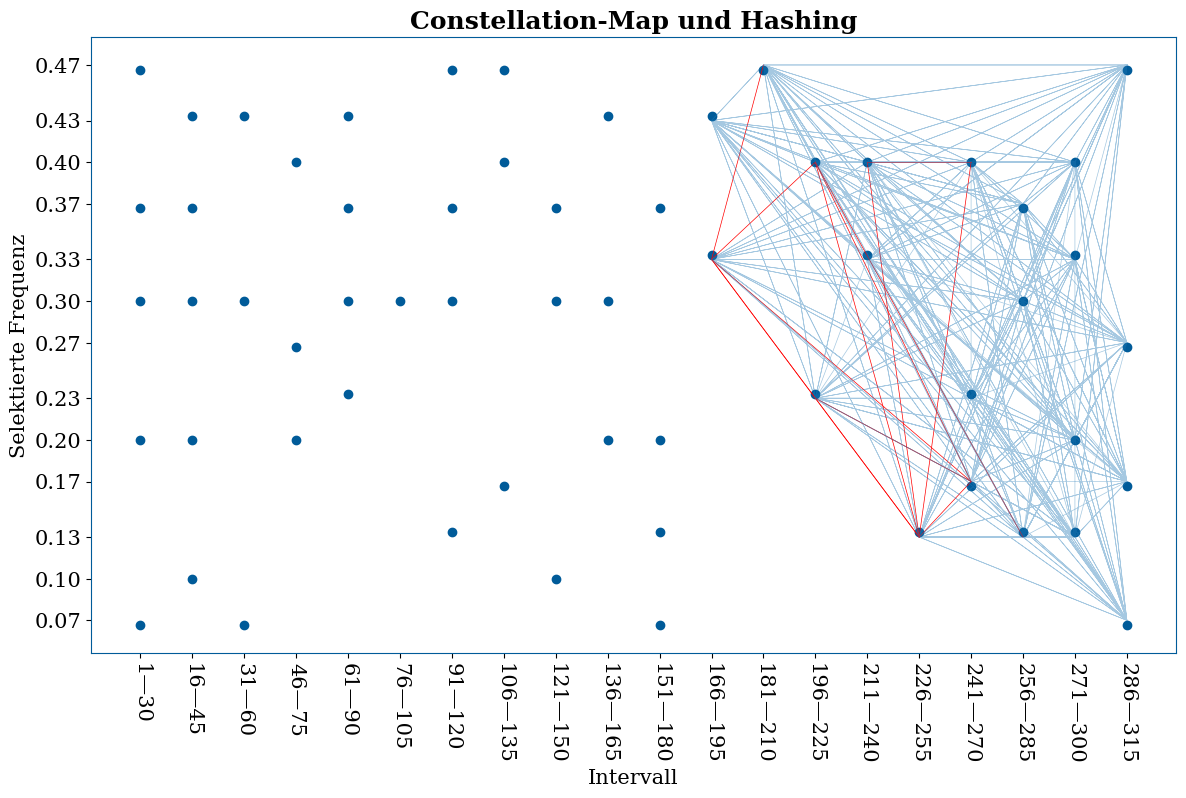
\includegraphics[width=1\textwidth]{plot_method.png}
            \caption{Constellation-Map und Hashing: Die Punkte bilden die Constellation-Map. Die zur Übersicht nur rechts eingezeichneten Kanten repräsentieren die Hash-Bildung, wobei rote Kanten ignorierte Hashes darstellen, weil sie mehrfach auftauchen.}
            \label{fig:hashing}
        \end{figure}

        Die Hashfunktion ist bijektiv gestaltet, sodass aus einem Hash all seine Bestandteile, die für die Erstellung verwendet wurden, eindeutig abgeleitet werden können. Das hängt damit zusammen, dass diese Bestandteile auf Bit-Ebene hintereinandergereiht werden, nämlich nach folgendem Schema:

        \begin{table}[H]
            \newcommand{\Col}[2]{\multicolumn{1}{|@{}p{#1\linewidth}@{}|}{\centering #2}}
            \centering
            \begin{tabular}{@{}p{0.125\linewidth}@{}p{0.5625\linewidth}@{}p{0.15625\linewidth}@{}p{0.15625\linewidth}@{}}
            % \begin{tabular}{|@{}p{0.125\linewidth}@{}|@{}p{0.5625\linewidth}@{}|@{}p{0.15625\linewidth}@{}|@{}p{0.15625\linewidth}@{}|}
                \hline
                \Col{0.125}{ 4 Bit} & \Col{0.5625}{18 Bit} & \Col{0.15625}{5 Bit} & \Col{0.15625}{5 Bit}\\
                \hline
                \centering Kidera Faktor & \centering Kantenlänge/Fensterabstand & \centering Frequenz Nachfolger & \centering Frequenz Ursprung
                % 4 Bit & 18 Bit & 5 Bit & 5 Bit\\
            \end{tabular}
        \end{table}

        Für 10 Faktoren reichen 4 Bit. Die Fenstergrößen belaufen sich auf unter 64, sodass mit 5 Bit alle möglichen Frequenzen abgedeckt werden können. Da die Anzahl Frequenzen immer gleich ist, können diese aufsteigend durchnummeriert werden, sodass die x-Achse in \autoref{fig:freq_selection} der Folge von 0 bis 15 entspräche. Die restlichen 18 Bit zu einem 32-Bit Integer dienen der ``Kantenlänge'' eines Hashes, auch wenn dafür bei den recht kurzen Sequenzen schon weniger als die Hälfte an Bits ausreichen würde, denn so viele Fenster sind gar nicht möglich, um die Kapazität voll auszuschöpfen.

        % Erstellung der Datenbank
        \begin{algorithm}[H]
            \caption{Erstellung der Datenbank}\label{alg:datenbank}
            \PhantomSubSub{Erstellung der Datenbank}
            \begin{algorithmic}
                \Require $fasta$ is a FASTA-formatted file
                \Ensure $database$ is a HashMap of: $Int \rightarrow Array\ of\ (Int, String)$

                \State $database \gets \texttt{hashmap}()$
                \ForEach{$protein\_id, sequence$}{$fasta$}
                    \For{$kf \gets 0\ \textbf{to}\ 10$}
                        \State $aa\_vector \gets \texttt{get\_aa\_vector}(sequence, kf)$
                        \State $constellation\_map \gets \texttt{get\_constellation\_map}(aa\_vector)$
                        \State $hashes \gets \texttt{get\_hashes}(constellation\_map, protein\_id)$
                        \ForEach{$hash$}{$hashes$}
                            \If{$hash\ \textbf{not in}\ database$}
                                \State $database[hash] \gets \texttt{array}()$
                            \EndIf
                            \State $database[hash].\texttt{append}(hashes[hash])$
                        \EndFor
                    \EndFor
                \EndFor
                \State $\texttt{save\_to\_file}(database)$
            \end{algorithmic}
        \end{algorithm}

        Die ersten drei beschriebenen Algorithmen beschreiben den Weg von einer Aminosäuresequenz in Textform zu den Hashes, die die strukturelle Information des Proteins entsprechend der spektralen Zerlegung mittels \ac{STFT} repräsentieren sollen. Übrig bleibt nur der Schritt, der die Hashes einer Menge von mehreren Proteinen in einer Datenbank vereinigt, sodass im Anschluss die Identifizierung von Eingabesequenzen erfolgen kann. Dafür werden je \ac{TP} für alle Kidera-Faktoren die Hashes gebildet und in die Datenbank geschrieben, welche eine HashMap ist. Im Gegensatz zu der resultierenden HashMap in \autoref{alg:hashing} verweisen die Hashes in der Datenbank allerdings nicht auf eine Position des Hashes für ein Protein, sondern auf eine Liste von solchen. Das heißt, dass für die Datenbank ein neuer Hash mit einem leeren Array initialisiert wird, in das darauf all diese Position-Protein\_ID-Tupel eingefügt werden.

        % hierzu ein Plot zur Veranschaulichung der Offsets
        % Scoring/Map-Vergleich
        Wurde die Datenbank erstellt, ist sie für die Identifizierung funktionsähnlicher Proteine anhand einer Eingabe verwendbar. Hierfür gibt es zwei Ansätze:
        \begin{enumerate}[a)]
            \item \PhantomSubSub{Single-Protein-Matching}
                \textbf{Single-Protein-Matching:}\ \ Eingabe ist eine FASTA-Datei, also eine Menge an Suchsequenzen. Ausgabe je Sequenz ist eine Liste von Treffern, sortiert nach Übereinstimmung der Hashes der Constellation-Maps von Treffer und Suchsequenz. Je höher der Rang eines Treffers, desto funktionsähnlicher sollte das entsprechende Protein sein. Die Ausgabe sind \ac{CSV}, also eine durch Kommata separierte Tabelle, mit folgenden Spalteninhalten:
            \begin{enumerate}[1.]
                \item Rank $\rightarrow$ Rang
                \item Match\_Protein\_ID $\rightarrow$ Protein-ID des Treffers
                \item JSI $\rightarrow$ Jaccard Similarity Index (siehe \autoref{alg:scoring})
                \item Score $\rightarrow$ Score (Übereinstimmung der Constellation-Map)
                \item Input\_Protein\_ID $\rightarrow$ Protein-ID der Suchsequenz
                \item Input\_Sequence\_Length $\rightarrow$ Sequenzlänge der Suchsequenz
                \item Input\_Found\_Hashes $\rightarrow$ Anzahl Hashes der Suchsequenz
            \end{enumerate}

            \newcommand{\Width}{\dimexpr\textwidth-\leftmargin}
            \begin{minipage}{\Width}
                \begin{algorithm}[H]
                    \caption{Treffer-Bewertung beim Single-Protein-Matching}\label{alg:scoring}
                    \begin{algorithmic}
                        \Require $hashes$ aus \autoref{alg:hashing}
                        \Require $database$ aus \autoref{alg:datenbank}
                        \Ensure $match\_scores$ is a HashMap of: $String \rightarrow Float$

                        \State $matches\_per\_tp \gets \texttt{hashmap}()$
                        \ForEach{$hash, position$}{$hashes$}
                            \If{$hash\ \textbf{in}\ database$}
                                \ForEach{$tp\_position, protein\_id$}{$database[hash]$}
                                    \If{$protein\_id\ \textbf{not in}\ matches\_per\_tp$}
                                        \State $matches\_per\_tp[protein\_id] \gets \texttt{hashmap}()$
                                    \EndIf
                                    \State $offset \gets tp\_position - position$
                                    \If{$offset\ \textbf{not in}\ matches\_per\_tp[protein\_id]$}
                                        \State $matches\_per\_tp[protein\_id][offset] \gets 0$
                                    \EndIf
                                    \State $offset\_count \gets matches\_per\_tp[protein\_id][offset]$
                                    \State $matches\_per\_tp[protein\_id][offset] \gets offset\_count + 1$
                                \EndFor
                            \EndIf
                        \EndFor
                        \State $match\_scores \gets \texttt{hashmap}()$
                        \ForEach{$protein, offsets$}{$matches\_per\_tp$}
                            \State $score \gets \texttt{get\_most\_common\_offset}(offsets)$
                            \State $match\_protein\_hashes \gets database.\texttt{get\_hashes}(protein)$
                            \State $jsi \gets \texttt{get\_jsi}(hashes, match\_protein\_hashes)$

                            \State $match\_scores[protein] \gets score \cdot jsi$
                        \EndFor
                    \end{algorithmic}
                \end{algorithm}
            \end{minipage}

            Um den Score zu bestimmen, also die Ähnlichkeit der Constellation-Map der Eingabe mit denen der \ac{TP}, werden pro Eingabe-Hash die Differenzen zwischen dessen Position mit den Positionen der trainierten Hashes gebildet und global pro Protein gezählt. Diese Differenzen repräsentieren den Abstand/Offset der Kante in der Eingabe-Map zur Kante der jeweiligen \ac{TP}-Map, also wie weit die Eingabe-Map verschoben wäre, sollte es sich bei dem \ac{TP} um das Original handeln. Auf diese Weise sammeln sich pro \ac{TP} mehrere solcher potentiellen Abstände, wobei der Abstand, der am häufigsten aufgetreten ist, offensichtlich die meiste Übereinstimmung in den Kanten zeigt. Diese Tatsache qualifiziert diese Maximalanzahl als geeigneten Score (S1) für ein Match.

            \begin{minipage}{\Width}
            \begin{figure}[H]
                \centering
                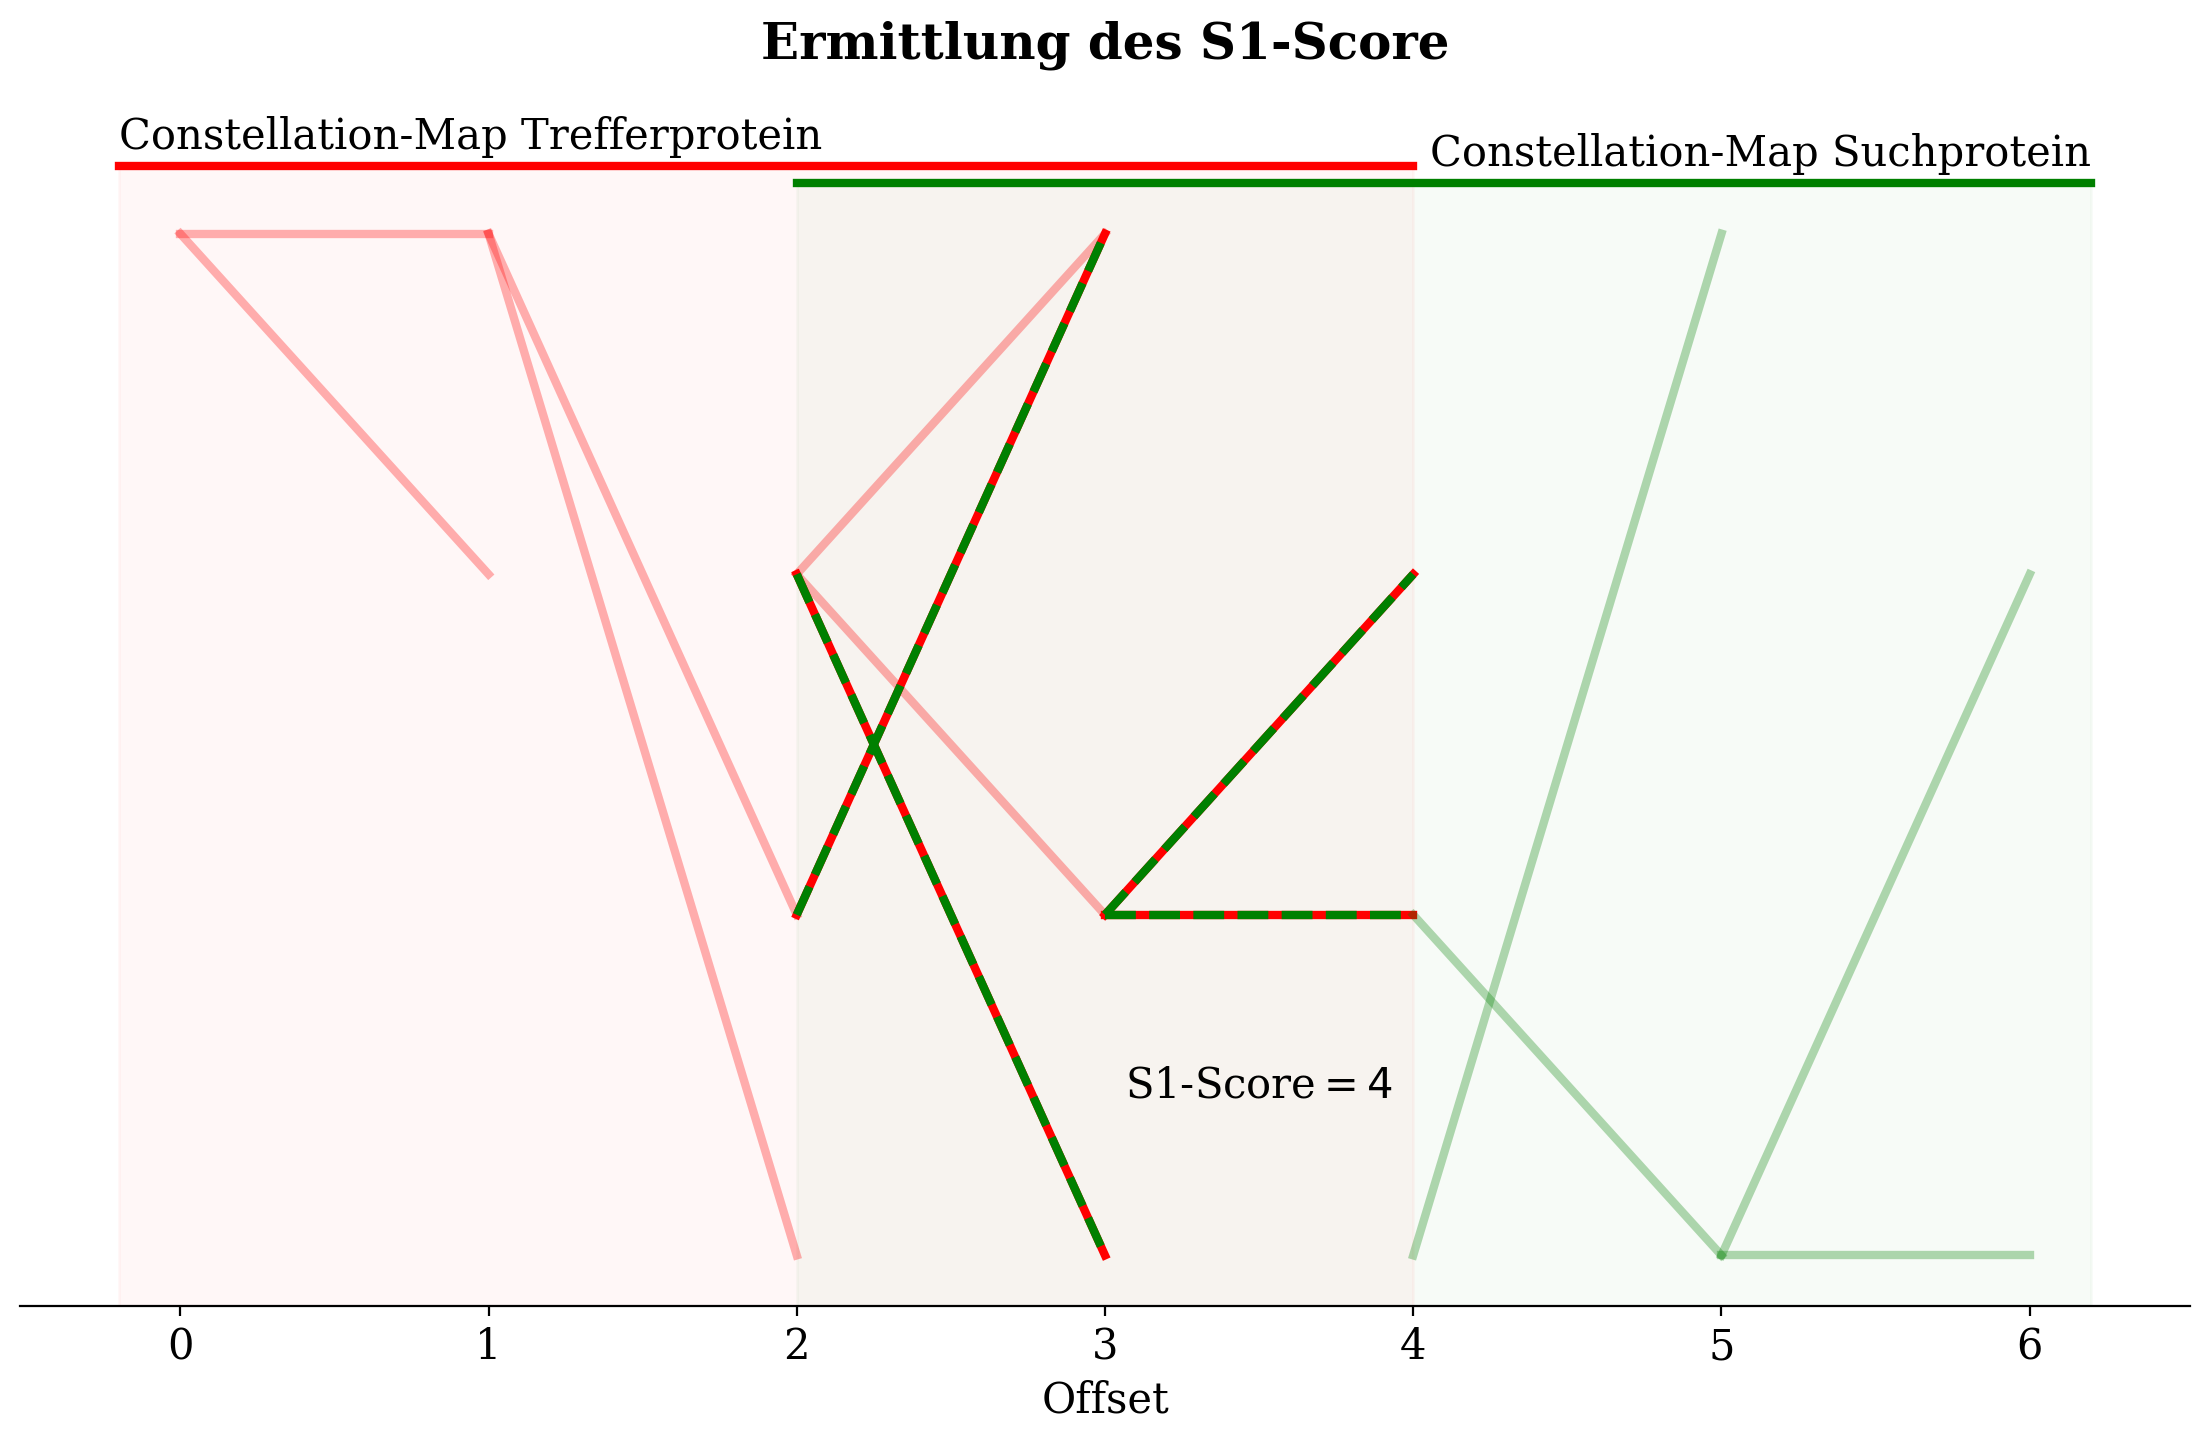
\includegraphics[width=\Width]{plot_scoring.png}
                \caption{Ermittlung des S1-Score: Die Constellation-Maps werden aneinander verschoben. Die maximale Überschneidung ist der Score.}
                \label{fig:scoring}
            \end{figure}
            \end{minipage}

            Da es große Proteine mit sehr langen Aminosäuresequenzen kürzere Sequenzen kleinerer funktionsungleicher Proteine enthalten können, reicht der ermittelte Score alleine nicht aus, da in diesem Fall sehr viele Kanten der Eingabe-Map übereinstimmen würden, sodass trotz Mis-Match der nahezu maximale Score erreicht werden würde. Bezogen auf das Beispiel zu S1 in \autoref{fig:scoring}, wäre dort der grüne Bereich vollständig vom roten Bereich eingeschlossen mit Überschneidungen in beinahe allen Kanten.

            Um das zu umgehen, wird der \ac{JSI} verwendet, einem Maß, das die Übereinstimmung zweier Mengen A und B wie folgt bewertet:
            $$JSI(A, B)=\frac{|A \cap B|}{|A \cup B|}$$
            Dieser Index nimmt einen Wert von 0 an, wenn beide Mengen disjunkt sind, und nähert sich der 1 je größer die Schnittmenge ist. Im Fall des Vergleichs zweier Constellation-Maps, also zwei Hash-Mengen, wird hier bewertet, wie viele Kanten sich die beiden Maps positionsunabhängig teilen. Durch diese Unabhängigkeit reicht der JSI alleine nicht als Score aus, sodass nur in Kombination/Multiplikation mit dem S1 ein robuster Score entsteht, da beide zusammen ihre Schwächen aufheben. Der \ac{JSI} in \autoref{fig:scoring} beträgt $\frac{4}{14} \approx 0.286$, da die Schnittmenge beider Hashmengen hier gleichzeitig den S1-Score bilden und die restlichen Hashes disjunkt zueinander sind. Der S1 wäre nur noch 3, wenn eine der markierten Kanten an einer anderen Position wäre, wobei der \ac{JSI} davon unberührt bliebe.

            \item \PhantomSubSub{Family-Matching}
                \textbf{Family-Matching:}\ \ Eingabe ist eine \ac{CSV}-Tabelle mit der Zuordnung von Protein-ID und -familie. Die für das Matching verwendeten Hashes sind hier diejenigen, die sich alle Mitglieder einer Suchfamilie teilen. Die Idee dahinter ist, dass diese Hashes spezifisch für diese Familie, beziehungsweise deren Funktion ist. Als Bewertungsmaß wird dabei die Anzahl Hashes des Treffers, die mit den Familienhashes übereinstimmen.

            Für die Ausgabe werden diese Treffer zusammengefasst. Dazu gibt es zwei Kriterien, den F-Score und die Schärfe (Sharpness), die nach folgender Berechnung ermittelt werden:
            \begin{equation}
                \begin{split}
                    t & = \texttt{max\_score}(TrP)\\
                    Sharpness & = \begin{cases}
                                      \frac{t-\texttt{max\_score}(FP)}{t},& \text{if t} > 0\\
                                      \sminus 1,& \text{sonst}
                                  \end{cases}\\
                    Precision & = \frac{|TrP|}{|TrP|+|FP|}\\
                    Recall & = \frac{|TrP|}{|TrP|-member\_count}\\
                    F\_Score & = \frac{2 \cdot Precision \cdot Recall}{Precision + Recall}
                \end{split}
            \end{equation}

            TrP ist hierbei die Menge der Treffer, die tatsächlich in der Familie vorkommen (true positives), wobei FP diejenigen sind, die das nicht tun (false positives) und einen besseren Score als der letzte korrekte Treffer haben. ``member\_count'' ist die Anzahl an Mitgliedern der Familie.

            Die Schärfe stellt das Verhältnis der besten Scores von FP und TrP dar, also wie weit der beste korrekte Treffer im Score von dem besten falschen Treffer entfernt ist.

            Die Präzision gibt an, wie viele der Treffer korrekt gewesen sind, während der Recall zeigt, wie viele der Familienmitglieder gefunden wurden. Der F-Score bringt diese beiden Werte zusammen.

            Die Ausgabe als \ac{CSV}-Tabelle beinhaltet aktuell diese Zusammenfassung zu Entwicklungszwecken. Sollte \protfin\ ausgereift sein, wird die Ausgabe vermutlich die Treffer je Suchfamilie enthalten. In den Spalten wird folgendes dokumentiert:
            \begin{enumerate}[1.]
                \item Family\_ID $\rightarrow$ ID der Suchfamilie
                \item F\_Score
                \item Precision
                \item Recall
                \item Sharpness 
                \item Member\_Count $\rightarrow$ Anzahl der Mitglieder der Suchfamilie
                \item Match\_Count $\rightarrow$ Anzahl gefundener Treffer
                \item Hash\_Intersec\_Size $\rightarrow$ Anzahl der Hashes, die sich die Mitglieder teilen
            \end{enumerate}
        \end{enumerate}

    % subsection grundalgorithmus (end)
    \subsection{Experiment 1: UniRef90 Sampling} % (fold)
        \label{sub:experiment_1_uniref90_sampling}
        Ein wichtiger Bestandteil des \hyperref[sec:grundalgorithmus]{Algorithmus} ist die Selektion signifikanter Frequenzen zur Erstellung der Constellation-Map. Es wäre möglich, einfach alle Frequenzen auszuwählen und die Signalstärke in den Hash einfließen zu lassen. Problem hierbei ist aber, dass diese Vorgehensweise zu wesentlich mehr Hashes und einer folglich sehr großen Datenbank führt, was wiederum das Scoring/Matching verlangsamt. Ein Anspruch an \protfin\ ist, dass die Datenbankgröße die Eingabegröße nicht wesentlich übersteigt, wobei es sich bei der Eingabe um eine einfache FASTA-Datei handelt.

        Diesem Problem soll durch ein Sampling-Experiment abgeholfen werden. Darin werden aus etwa 180 Millionen Sequenzen je ein zufälliges Fenster fester Größe für die \ac{STFT} ausgewählt, transformiert und die Signalstärken je Frequenz gemerkt. Um daraus eine Selektionsmethode abzuleiten, werden die Grenzquantile einer jeden Frequenz ermittelt, um signifikant seltene Signalstärken zu ermitteln. Folglich ist es möglich, für die Constellation-Map nur diejenigen Frequenzen zu behalten, welche in den Randzonen der Signalstärken liegen, sodass nicht nur Signale infrage kommen, die für eine besonders starke Ausprägung eines Kidera-Faktors sprechen, sondern auch für den Fall der umgekehrten Ausprägung, wie z.B. Hydrophilie statt Hydrophobie.

        Der Algorithmus wird daher insofern angepasst, dass bei der Frequenz-Selektion von den Maxima der Signalstärken nur die behalten werden, die die Grenzwerte über- oder unterschreiten. Zudem wird beim Hashing je Frequenz noch die Information hinzugefügt, ob sie besonders stark oder schwach ist.
    
    % subsection experiment_1_uniref90_sampling (end)
% section material_und_methoden (end)
